
\begin{frame}
    \frametitle{¿Pero qué es la ADVUCA?}
    
    \begin{center}
        \begin{alertblock}{¡Es un acrónimo!}
            \emph{ADVUCA} $\rightarrow$ Asociación de Desarrollo de Videojuegos de la UCA
        \end{alertblock}        
    \end{center}
    
    \begin{columns}[c]
		\column{150pt}
		\begin{block}{La fundamos}
            \begin{itemize}
                \item David Saltares Márquez
                \item Jose Marente Florín
                \item Alberto Cejas Sánchez
                \item Francisco Javier Santacruz López-Cepero
                \item Sebastián Guerrero Selma
            \end{itemize}            
        \end{block}
	\begin{center}
	    Somos alumnos de la ESI
	\end{center}
		\column{150pt}
		\begin{center}
			
\includegraphics[scale=0.2]{img/advuca.png}
		\end{center}
	\end{columns} 
\end{frame}

	
\begin{frame}
	\frametitle{Nuestros objetivos}
	
	\begin{columns}[c]
		\column{75pt}
		\begin{center}
			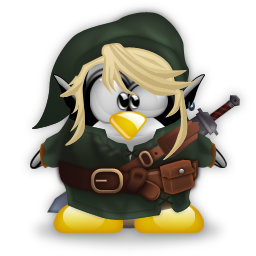
\includegraphics[scale=0.3]{img/link.png}
		\end{center}
		\column{225pt}
		
		\begin{center}
			Este taller es sólo el principio
		\end{center}		
		
		\begin{block}{Pretendemos}
            \begin{itemize}
                \item Formar grupos de desarrollo de videojuegos
				\item Ofrecer documentación sobre creación de videojuegos
				\item Colaborar con asignaturas de la carrera
				\item Trabajo con grupos interdisciplinares (programación, grafismo, sonido...)
				\item ¡Divertirnos!
            \end{itemize}            
        \end{block}        
	\end{columns}
\end{frame}

\begin{frame}
	\frametitle{Inscríbete}
	
	\begin{columns}[c]
		\column{150pt}
	
	http://blog.advuca.com
		
	\begin{block}{Sólo necesitas}
            \begin{itemize}
                \item Matrícula de la UCA
		\item Datos personales
		\item No pedimos pasta, sólo ganas de aprender ;-)
            \end{itemize}            
        \end{block}        
		\column{150pt}
		\begin{center}
			
\includegraphics[scale=0.22]{img/iwantyou.jpg}
		\end{center}
	\end{columns} 
	
\end{frame}
